\documentclass[12pt,a4paper,twoside]{report}
\usepackage[a4paper,outer=1cm,inner=3cm,top=2cm,bottom=1cm]{geometry}
\usepackage{setspace}
\usepackage{polyglossia}
\usepackage{fontspec}
\usepackage{xltxtra}
\usepackage{listings}
\usepackage{titlesec}
\usepackage{color}
\usepackage{xcolor}

\defaultfontfeatures{Scale=MatchLowercase}
\setsansfont[Mapping=tex-text]{Helvetica}
\renewcommand*{\familydefault}{\sfdefault}

\usepackage{amsmath}
\usepackage{amsfonts}

\newcommand{\ch}{\operatorname{ch}}
\newcommand{\sh}{\operatorname{sh}}

\titleformat{\section}{\normalfont\fontsize{25}{25}\bfseries\centering}{\thesection}{1em}{}
\newcommand{\sectionbreak}{\clearpage}

\title{
	Компьютерный праткикум по\\
	линейной алгебре.\\
	Расчётное задание №2\\[4em]
}
\author{Вилков Кирилл Олегович, группа 14ПИ}
\date{12.01.15}

\makeatletter
\def\Title{Расчётное задание №1}
\let\theauthor\@author
\makeatother

\usepackage{fancyhdr}
\pagestyle{fancy}
\fancyhf{}
\fancyhead[LE,RO]{\thepage}
\fancyhead[RE,LO]{\Title \qquad \theauthor}
\fancyheadoffset{0mm}
\fancyfootoffset{0mm}
\setlength{\headheight}{15pt}
\renewcommand{\headrulewidth}{1pt}
\renewcommand{\footrulewidth}{0pt}

\usepackage{tocloft}

\setcounter{tocdepth}{1}
\setcounter{secnumdepth}{0}
\renewcommand\contentsname{Содержание}
\tocloftpagestyle{fancy}

\usepackage{listings}
%\usepackage{courier}

\definecolor{dkgreen}{rgb}{0,0.6,0}
\definecolor{gray}{rgb}{0.5,0.5,0.5}
\definecolor{mauve}{rgb}{0.58,0,0.82}

\lstset{
	frame=tb,
	xleftmargin=20pt,
	language=Matlab,
	aboveskip=3mm,
	belowskip=3mm,
	showstringspaces=false,
	columns=flexible,
	basicstyle={\small\ttfamily},
	numbers=none,
	breaklines=true,
	breakatwhitespace=true
	tabsize=2
}

\newcommand{\showcode}[1]{
	%\begin{minipage}{\linewidth}
		\lstinputlisting{#1}
	%\end{minipage}
}
\newcommand{\showscreen}[1]{
\\ \includegraphics[scale=0.6]{#1} \\
}


\begin{document}

	\maketitle
	\pagestyle{fancy}
	\setcounter{page}{1}
	\tableofcontents
	\newpage

	\renewcommand*{\arraystretch}{1.5}

	\section{Задача 1.24}
\subsection{Задание:}
Решить
$
	\left|
		\begin{matrix}
			2 & x & 6 \\
			3 & 3 & 9 \\
			7 & 4 & 11
		\end{matrix}
	\right|
	= 0
$
\subsection{Решение:}
$
	3 \cdot 11 \cdot x + 2 \cdot 4 \cdot 9 + 2 \cdot 3 \cdot 11 -
	6 \cdot 3 \cdot 4 - 6 \cdot 3 \cdot 7 - 7 \cdot 9 \cdot x = 0
	\\[1ex]
	-30x - 60 = 0
	\\[1ex]
	x = -\dfrac{60}{30} = 2
$
\subsection{Проверим результат в среде Wolfram Mathematica:}
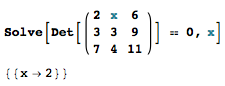
\includegraphics[scale=0.6]{task/1_24/screen.png}
\subsection{Ответ:}
Компьютерная проверка подтвердила полученный результат.

	\section{Задача 1.25}
\subsection{Задание:}
Найти матрицу обратную к
$
	A =
	\begin{pmatrix}
		2 & 4 & 0 & 1 \\
		3 & -3 & 5 & 0 \\
		-1 & 0 & 1 & 1 \\
		2 & 1 & 1 & 0 \\
	\end{pmatrix}
$
\; методом алгебраических дополненй.
\subsection{Решение:}
Найдём $ \det A $ чтобы убедиться что $ \exists A^{-1} $:
\\[1em]
$
	\det A =
	\begin{vmatrix}
		2 & 4 & 0 & 1 \\
		3 & -3 & 5 & 0 \\
		-1 & 0 & 1 & 1 \\
		2 & 1 & 1 & 0 \\
	\end{vmatrix}
	=
	\begin{vmatrix}
		3 & 4 & -1 & 0 \\
		3 & -3 & 5 & 0 \\
		-1 & 0 & 1 & 1 \\
		2 & 1 & 1 & 0 \\
	\end{vmatrix}
	=
	\begin{vmatrix}
		3 & 4 & -1 & 0 \\
		3 & -3 & 5 & 0 \\
		-1 & 0 & 1 & 1 \\
		2 & 1 & 1 & 0 \\
	\end{vmatrix}
	=
	-
	\begin{vmatrix}
		3 & 4 & -1 \\
		3 & -3 & 5 \\
		2 & 1 & 1 \\
	\end{vmatrix}
	=
	5
$
\\[1em]
$ \det A \neq 0 \Rightarrow \exists A^{-1} = \dfrac{D^T}{\det A} $
\\[1em]
$
	d_{11} =
	\begin{vmatrix}
		-3 & 5 & 0 \\
		0 & 1 & 1 \\
		1 & 1 & 0 \\
	\end{vmatrix}
	=
	\begin{vmatrix}
		-3 & 5 & 0 \\
		0 & 1 & 1 \\
		1 & 1 & 0 \\
	\end{vmatrix}
	=
	-
	\begin{vmatrix}
		-3 & 5 \\
		1 & 1 \\
	\end{vmatrix}
	= 8
\\[1em]
	d_{12} =
	\begin{vmatrix}
		3 & 5 & 0 \\
		-1 & 1 & 1 \\
		2 & 1 & 0 \\
	\end{vmatrix}
	=
	-
	\begin{vmatrix}
		3 & 5 \\
		2 & 1 \\
	\end{vmatrix}
	=
	7
\\[1em]
	d_{13} =
	\begin{vmatrix}
		3 & -3 & 0 \\
		-1 & 0 & 1 \\
		2 & 1 & 0 \\
	\end{vmatrix}
	=
	-
	\begin{vmatrix}
		3 & -3 \\
		2 & 1 \\
	\end{vmatrix}
	=
	-9
\\[1em]
	d_{14} =
	\begin{vmatrix}
		3 & -3 & 5 \\
		-1 & 0 & 1 \\
		2 & 1 & 1 \\
	\end{vmatrix}
	=
	\begin{vmatrix}
		-3 & 5 \\
		1 & 1 \\
	\end{vmatrix}
	-
	\begin{vmatrix}
		3 & -3 \\
		2 & 1 \\
	\end{vmatrix}
	=
	-8 - 9 = -17
\\[1em]
	d_{21} =
	\begin{vmatrix}
		4 & 0 & 1 \\
		0 & 1 & 1 \\
		1 & 1 & 0 \\
	\end{vmatrix}
	=
	4
	\begin{vmatrix}
		1 & 1 \\
		1 & 0
	\end{vmatrix}
	+
	\begin{vmatrix}
		0 & 1 \\
		1 & 1
	\end{vmatrix}
	= -4 - 1 = -5
\\[1em]
	d_{22} =
	\begin{vmatrix}
		2  & 0 & 1 \\
		-1 & 1 & 1 \\
		2 & 1 & 0 \\
	\end{vmatrix}
	=
	2
	\begin{vmatrix}
		1 & 1 \\
		1 & 0 \\
	\end{vmatrix}
	+
	\begin{vmatrix}
		-1 & 1 \\
		2 & 1 \\
	\end{vmatrix}
	= -2 - 3 = -5
\\[1em]
$

	\section{Задача 1.26}
\subsection{Задание:}
Решить систему линейных уравнений методом Крамера в компьютерной среде
\\[1em]
$
	\begin{cases}
		3x_1 + 2x_2 + x_3 = 5  \\
		2x_1 + 3x_2 + x_3 = 1  \\
		2x_1 + x_2 + 3x_3 = 11 \\
	\end{cases}
$
\subsection{Решение:}
Решим СЛУ в системе Wolfram Mathematica:
Найдём $ \Delta $:
\\
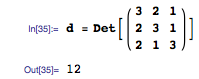
\includegraphics[scale=0.6]{task/1_26/screen1.png}
\\
Найдём $ \Delta_1, \Delta_2, \Delta_3 $:
\\
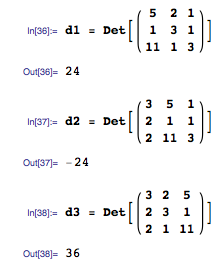
\includegraphics[scale=0.6]{task/1_26/screen2.png}
\\
Найдём корни уравнения:
\\
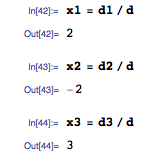
\includegraphics[scale=0.6]{task/1_26/screen3.png}
\\
\subsection{Вывод:}
Мы нашли решение системы методом Крамера: $ x_1 = 2, x_2 = -2, x_3 = 3 $.

	\section{Задача 1.27}
\subsection{Задание:}
Не вычисляя определитель
$
	\begin{vmatrix}
		2 & 1 & 7 & 8 & 1 \\
		3 & 9 & 7 & 7 & 4 \\
		6 & 5 & 3 & 4 & 3 \\
		8 & 0 & 4 & 9 & 5 \\
		7 & 2 & 9 & 1 & 9 \\
	\end{vmatrix}
$
доказать что он делится нацело на 947.
\subsection{Решение:}
По свойству определителя к любомоу столбцу можно прибавить линейную комбинацию других, и определитель не изменится.
Прибавим к последнему столбцу линейную комбинацию других:
\\
$
	\tilde a_{\bullet 5} =
	10000 \cdot a_{\bullet 1} +
	1000  \cdot a_{\bullet 2} +
	100   \cdot a_{\bullet 3} +
	10    \cdot a_{\bullet 4}
	+ a_{\bullet 5}
$
\\
Тогда определитель принимает вид:
\\[1em]
$
	\begin{vmatrix}
		2 & 1 & 7 & 8 & 21781 \\
		3 & 9 & 7 & 7 & 39774 \\
		6 & 5 & 3 & 4 & 65343 \\
		8 & 0 & 4 & 9 & 80495 \\
		7 & 2 & 9 & 1 & 72919 \\
	\end{vmatrix}
	=
	947 \cdot
	\begin{vmatrix}
		2 & 1 & 7 & 8 & 23 \\
		3 & 9 & 7 & 7 & 42 \\
		6 & 5 & 3 & 4 & 69 \\
		8 & 0 & 4 & 9 & 85 \\
		7 & 2 & 9 & 1 & 77 \\
	\end{vmatrix}
$
\\[1em]
Значит определитель делится нацело на 947
\subsection{Компьютерная проверка в среде Wolfram Mathematica:}
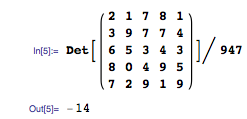
\includegraphics[scale=0.6]{task/1_27/screen1.png}
\subsection{Вывод:}
Компьютерная проверка показала что определитель действительно делится нацело на 947.

	\section{Задача 1.31}
\subsection{Задание:}
Вычислить
$
	\begin{vmatrix}
		1 & 2 & 3 & \cdots & n - 1 & n \\
		-1 & 0 & 3 & \cdots & n - 1 &  n \\
		-1 & -2 & 0 & \cdots & n - 1 & n \\
		\vdots & \vdots & \vdots & \ddots & \vdots & \vdots \\
		-1 & -2 & -3 & \cdots & -(n - 1) & 0 \\
	\end{vmatrix}
$.
\subsection{Решение:}
Вынесем общий множитель из каждого столбца определителя (вынесем из каждого столбца номер этого столбца),
тогда определитель принимает вид:
\\[1em]
$
	n! \cdot
	\begin{vmatrix}
		1 & 1 & 1 & \cdots & 1 & 1 \\
		-1 & 0 & 1 & \cdots & 1 &  1 \\
		-1 & -1 & 0 & \cdots & 1 & 1 \\
		\vdots & \vdots & \vdots & \ddots & \vdots & \vdots \\
		-1 & -1 & -1 & \cdots & -1 & 0 \\
	\end{vmatrix}
$
\\[1em]
Докажем методом мат. индукции что
$
	\begin{vmatrix}
		1 & 1 & 1 & \cdots & 1 & 1 \\
		-1 & 0 & 1 & \cdots & 1 &  1 \\
		-1 & -1 & 0 & \cdots & 1 & 1 \\
		\vdots & \vdots & \vdots & \ddots & \vdots & \vdots \\
		-1 & -1 & -1 & \cdots & -1 & 0 \\
	\end{vmatrix}
	= 1
$
\\[1em]
Проверим базу $ n = 1 $: $ |1| = 1 $
\\
Предположим что утверждение верно для $ n $, тогда докажем для $ n + 1 $:
\\[1em]
$
	\begin{vmatrix}
		1 & 1 & 1 & \cdots & 1 & 1 \\
		-1 & 0 & 1 & \cdots & 1 &  1 \\
		-1 & -1 & 0 & \cdots & 1 & 1 \\
		\vdots & \vdots & \vdots & \ddots & \vdots & \vdots \\
		-1 & -1 & -1 & \cdots & -1 & 0 \\
	\end{vmatrix}_{n + 1}
	=
	\begin{vmatrix}
		1 & 1 & 1 & \cdots & 1 & 1 \\
		-1 & 0 & 1 & \cdots & 1 &  1 \\
		-1 & -1 & 0 & \cdots & 1 & 1 \\
		\vdots & \vdots & \vdots & \ddots & \vdots & \vdots \\
		0 & 0 & 0 & \cdots & 0 & 1 \\
	\end{vmatrix}_{n + 1}
	=
	1 \cdot
	\begin{vmatrix}
		1 & 1 & 1 & \cdots & 1 & 1 \\
		-1 & 0 & 1 & \cdots & 1 &  1 \\
		-1 & -1 & 0 & \cdots & 1 & 1 \\
		\vdots & \vdots & \vdots & \ddots & \vdots & \vdots \\
		-1 & -1 & -1 & \cdots & -1 & 0 \\
	\end{vmatrix}_{n}
$
\\[1em]
Утверждение доказано.
\\[1em]
Получается что
$
	\begin{vmatrix}
		1 & 2 & 3 & \cdots & n - 1 & n \\
		-1 & 0 & 3 & \cdots & n - 1 &  n \\
		-1 & -2 & 0 & \cdots & n - 1 & n \\
		\vdots & \vdots & \vdots & \ddots & \vdots & \vdots \\
		-1 & -2 & -3 & \cdots & -(n - 1) & 0 \\
	\end{vmatrix}
	=
	n!
$
\subsection{Компьютерная проверка:}
Выполним проверку в среде Wolfram Mathematica при $ n = 8 $:
\\
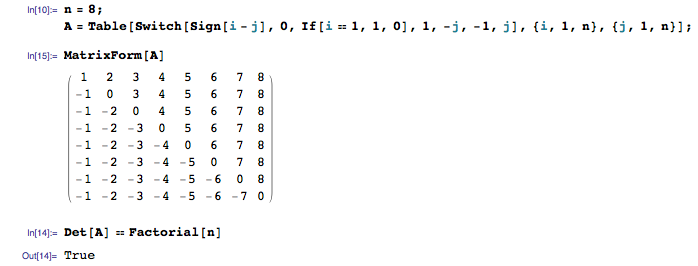
\includegraphics[scale=0.6]{task/1_31/screen1.png}
\subsection{Вывод:}
Компьютерная проверка подтвертила правильность полученной формулы.

	\section{Задача 1.33}
\subsection{Задание:}
Вычислить:
\\[1em]
$
	\begin{vmatrix}
		0 & 1 & 1 & 1 & \cdots & 1 & 1 \\
		1 & a_1 & 0 & 0 & \cdots & 0 & 0 \\
		1 & 0 & a_2 & 0 & \cdots & 0 & 0 \\
		\vdots & \vdots & \vdots & \vdots & \ddots & \vdots & \vdots \\
		1 & 0 & 0 & 0 & \cdots & a_{n-1} & 0 \\
		1 & 0 & 0 & 0 & \cdots & 0 & a_n \\
	\end{vmatrix}
$
\subsection{Решение:}
Можно заметить что для различных $ n $ определитель такой матрицы равен
$ |A| = -\sum \limits_{i=1}^n \dfrac{1}{a_i} \prod \limits_{i=1}^n a_i $
\\
Докажем методом математической индукции:
\\
При $ n = 2 $:
\\
$
	\begin{vmatrix}
		0 & 1 & 1 \\
		1 & a_1 & 0 \\
		1 & 0 & a_2 &
	\end{vmatrix}
	= -a_1 - a_2
$
\\
Если утверждение верно при $ n $, тогда при $ n + 1 $
\\
$
\begin{vmatrix}
	0 & 1 & 1 & 1 & \cdots & 1 & 1 \\
	1 & a_1 & 0 & 0 & \cdots & 0 & 0 \\
	1 & 0 & a_2 & 0 & \cdots & 0 & 0 \\
	\vdots & \vdots & \vdots & \vdots & \ddots & \vdots & \vdots \\
	1 & 0 & 0 & 0 & \cdots & a_{n} & 0 \\
	1 & 0 & 0 & 0 & \cdots & 0 & a_{n+1} \\
\end{vmatrix}
= (-1)^{n+2} \cdot (-1)^{n+1} \cdot
\begin{vmatrix}
	0 & 1 & 1 & 1 & \cdots & 1 & 1 \\
	1 & a_1 & 0 & 0 & \cdots & 0 & 0 \\
	1 & 0 & a_2 & 0 & \cdots & 0 & 0 \\
	\vdots & \vdots & \vdots & \vdots & \ddots & \vdots & \vdots \\
	1 & 0 & 0 & 0 & \cdots & a_{n-1} & 0 \\
	1 & 0 & 0 & 0 & \cdots & 0 & a_n \\
\end{vmatrix}
- \sum \limits_{i=1}^n \dfrac{1}{a_i} \prod \limits_{i=1}^{n+1} a_i =
- \sum \limits_{i=1}^{n+1} \dfrac{1}{a_i} \prod \limits_{i=1}^{n+1} a_i
$
\subsection{Выполним компьютерную проверку в среде Wolfram Mathematica:}
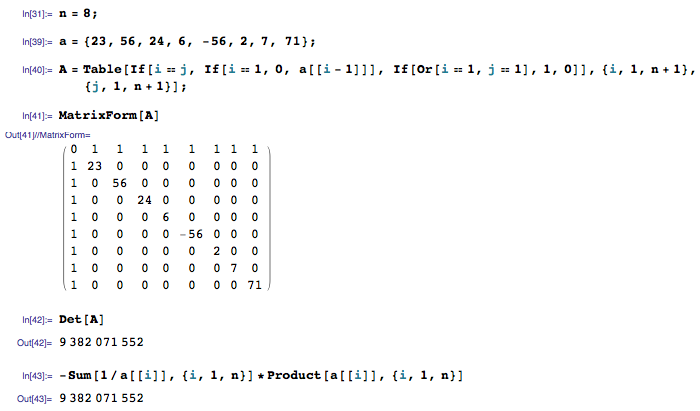
\includegraphics[scale=0.6]{task/1_33/screen.png}
\subsection{Вывод:}
Мы выполнили компьютерную проверку и убедились в верности предположения.

	\section{Задача 1.35}
\subsection{Задание:}
Вычислить $ \det A, A = \{ a_{ij} \} |, i = \overline{1,n}, j = \overline{1,n}, a_{ij} = \min (i,j) $
\subsection{Решение:}
Докажем методом мат. индукции что $ \det A = 1 $:
\\
Проверим базу индукции: $ |1| = 1 $
\\
Допустим что утверждение верно для $ n $, тогда докажем что оно будет верно для $ n + 1 $:
\\[1em]
$
	\begin{vmatrix}
		     1 &      1 & \cdots &      1 &       1 \\
		\vdots & \vdots & \ddots & \vdots &  \vdots \\
		     1 &      2 & \cdots &      n &       n \\
		     1 &      2 & \cdots &      n &   n + 1 \\
	\end{vmatrix}_{n + 1}
	=
	\begin{vmatrix}
		     1 &      1 & \cdots &      1 &       1 \\
		\vdots & \vdots & \ddots & \vdots &  \vdots \\
		     1 &      2 & \cdots &      n &       n \\
		     0 &      0 & \cdots &      0 &       1 \\
	\end{vmatrix}_{n + 1}
	=
	\begin{vmatrix}
		     1 &      1 & \cdots &      1  \\
		\vdots & \vdots & \ddots & \vdots  \\
		     1 &      2 & \cdots &      n  \\
	\end{vmatrix}_n
$
\\[1em]
В силу мат. индукции предположение доказано.
\subsection{Компьютерная проверка в среде Wolfram Mathematica:}
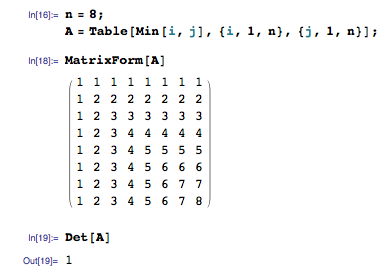
\includegraphics[scale=0.6]{task/1_35/screen1.png}
\subsection{Вывод:}
Компьютерная проверка показала что утверждение верно.

	\section{Задача 1.38}
\subsection{Задание:}
Как изменится определитель если в нём:\\
а) к каждой строке, кроме последней, прибавить последнюю строку;\\
б) из каждой строки, кроме последней, вычесть все последующие строки;\\
в) из каждой строки, кроме последней, вычесть последующую строку, а из последней вычесть бывшую первоначально первой;\\
г) повернуть его матрицу на $ 90 $ градусов вокруг центра по часовой стрелке;\\
д) первый столбец поставить на последнее место, сохранив порядок следования остальных столбцов.\\
\subsection{К каждой строке, кроме последней, прибавить последнюю строку:}
По свойству определителя если к любой строке определителя прибавить другую строку определителя, он не изменится.
Значит и в результате данного преобразования определитель не изменится.
\subsection{Из каждой строки, кроме последней, вычесть все последующие строки:}
По свойству определителя если к любой строке определителя прибавить линейную комбинацию других строк определителя, он не изменится.
Значит и в результате данного преобразования определитель не изменится.
\subsection{Из каждой строки, кроме последней, вычесть последующую строку, а из последней вычесть бывшую первоначально первой}
Пусть есть матрица $ A $ над которой мы будем производить такую операцию.
Эта операция равнозначна умножению слева матрицы $ A $ на матрицу
$
	B =
	\begin{pmatrix}
		1      & -1     & 0      & \cdots & 0      & 0      \\
		0      & 1      & -1     & \cdots & 0      & 0      \\
		\vdots & \vdots & \vdots & \ddots & \vdots & \vdots \\
		0      & 0      & 0      & \cdots & 1      & -1     \\
		-1     & 0      & 0      & \cdots & 0      & 1      \\
	\end{pmatrix}
$. По свойству определителя $ |BA| = |B| \cdot |A| $. Найдём $ |B| $ разложив его по последней строке:
\\[1em]
$
	B \in M(n)
	\\[1em]
	|B| = (-1)^{n+1} \cdot
	\begin{vmatrix}
		-1     & 0      & \cdots & 0      & 0      \\
		1      & -1     & \cdots & 0      & 0      \\
		\vdots & \vdots & \ddots & \vdots & \vdots \\
		0      & 0      & \cdots & 1      & -1     \\
	\end{vmatrix}
	+
	\begin{vmatrix}
		1      & -1     & 0      & \cdots & 0      \\
		0      & 1      & -1     & \cdots & 0      \\
		\vdots & \vdots & \vdots & \ddots & \vdots \\
		0      & 0      & 0      & \cdots & -1     \\
		0      & 0      & 0      & \cdots & 1      \\
	\end{vmatrix}
	=
	\\[1em]
	=
	(-1)^{n+1} \cdot (-1)^n + 1 = -1 + 1 = 0
$
\\[1em]
Тогда $ |BA| = 0 \cdot |A| = 0 $, в результате такого преобразования определеитель станет равен нулю.
\subsection{Повернуть его матрицу на $ 90 $ градусов вокруг центра по часовой стрелке}
Чтобы повернуть матрицу на $ 90 $ градусов транспонируем её, а потом умножим справа на матрицу
\\[1em]
$
	B =
	\begin{pmatrix}
		0 & \cdots & 0 & 1 \\
		0 & \cdots & 1 & 0 \\
		\vdots & \ddots & \vdots & \vdots \\
		1 & \cdots & 0 & 0 \\
	\end{pmatrix}
\\
	|B| = (-1)^{\left[\frac{n}{2}\right]}
$ значит изменённый определитель $ |A'| = (-1)^{\left[\frac{n}{2}\right]} \cdot |A| $
\subsection{Первый столбец поставить на последнее место, сохранив порядок следования остальных столбцов}
Для этого последовательно будем менять $ i $-ый и $ i+1 $-ый столбцы начиная с $ i = 1 $ до $ n - 1 $.
При каждой замене знак определителя будет меняться на противоположный, всего замен $ n - 1 $, значит $ |A'| = (-1)^{n-1} \cdot |A| $.

	\section{Задача 2.1}
\subsection{Задание:}
Вычислить
$
	\dfrac{(2 + 2i)^2 - (1 - i)^3}{(3 + 2i)^3 - (2 + i)^2}
$
\subsection{Решение:}
$
	\dfrac{(2 + 2i)^2 - (1 - i)^3}{(3 + 2i)^3 - (2 + i)^2}
	=
	\dfrac{8i + 2i}{-9 + 46i - 3 - 4i}
	=
	\dfrac{10i}{-12 + 42i}
	=
	\dfrac{35}{159} - \dfrac{17}{159} i
$
\subsection{Проверка в среде Wolfram Mathematica:}
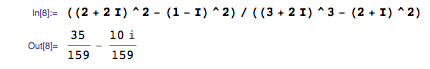
\includegraphics[scale=0.6]{task/2_01/screen1.png}
\subsection{Вывод:}
Мы вычилслили значение выражения и проверили результат в компьютерной среде.

	\section{Задача 2.2}
\subsection{Задание:}
Вычислить
$
	\dfrac{(1+i)^9}{(1-i)^9}
$
\subsection{Решение:}
$
	\dfrac{(1+i)^9}{(1-i)^9}
	=
	(\dfrac{(1+i)}{(1-i)})^9
	=
	(\dfrac{(1+i)(1+i)}{(1+i)(1-i)})^9
	=
	(\dfrac{1 - 2i - 1}{1 + 1})^9
	=
	\\[1em]
	=
	(-i)^{25}
	=
	(-i)^{24} \cdot i
	=
	(-1)^{12} \cdot i
	=
	1 \cdot i
	=
	i
$
\subsection{Компьютерная проверка в среде Wolfram Mathematica}
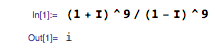
\includegraphics[scale=0.6]{task/2_02/screen1.png}
\subsection{Вывод:}
Мы правильно вычислили значение выражения.

	\section{Задача 2.3}
\subsection{Задание:}
$
	\begin{cases}
		(1 + i)x + (1 + 2i)y + (1 + 3i)z + (1 + 4i)t = 1 + 5i \\
		(3 - i)x + (4 - 2i)y + (1 + i)z + 4it = 2 - i
	\end{cases}
$
\subsection{Решение:}
Преобразуем систему:
\\[1em]
$
	\begin{cases}
		x + y + z + t = 1 \\
		3x + 4y + z = 2 \\
		ix + 2iy + 3iz + 4it = 5i \\
		-ix -2iy + iz + 4it = -i
	\end{cases}
$
\\[1em]
Разделим последние две строчки на $ i $:
\\[1em]
$
\begin{cases}
	x + y + z + t = 1 \\
	3x + 4y + z = 2 \\
	x + 2y + 3z + 4t = 5 \\
	-x -2y + z + 4t = -1
\end{cases}
$
\\[1em]
Решим систему методом Крамера:
\\[1em]
$
	\Delta =
	\begin{vmatrix}
		1 & 1 & 1 & 1 \\
		3 & 4 & 1 & 0 \\
		1 & 2 & 3 & 4 \\
		-1 & -2 & 1 & 4 \\
	\end{vmatrix} = 8
	\\[1em]
	\Delta_x =
	\begin{vmatrix}
		1 & 1 & 1 & 1 \\
		2 & 4 & 1 & 0 \\
		5 & 2 & 3 & 4 \\
		-1 & -2 & 1 & 4 \\
	\end{vmatrix} = -16
	\\[1em]
	\Delta_y =
	\begin{vmatrix}
		1 & 1 & 1 & 1 \\
		3 & 2 & 1 & 0 \\
		1 & 5 & 3 & 4 \\
		-1 & -1 & 1 & 4 \\
	\end{vmatrix} = 12
	\\[1em]
	\Delta_z =
	\begin{vmatrix}
		1 & 1 & 1 & 1 \\
		3 & 4 & 2 & 0 \\
		1 & 2 & 5 & 4 \\
		-1 & -2 & -1 & 4 \\
	\end{vmatrix} = 16
	\\[1em]
	\Delta_t =
	\begin{vmatrix}
		1 & 1 & 1 & 1 \\
		3 & 4 & 1 & 2 \\
		1 & 2 & 3 & 5 \\
		-1 & -2 & 1 & -1 \\
	\end{vmatrix} = -4
	\\[1em]
	x = \dfrac{\Delta_x}{\Delta} = -2 \\[1em]
	y = \dfrac{\Delta_y}{\Delta} = \dfrac{3}{2} \\[1em]
	z = \dfrac{\Delta_z}{\Delta} = 2 \\[1em]
	t = \dfrac{\Delta_t}{\Delta} = - \dfrac{1}{2} \\[1em]
$
\subsection{Выполним компьютерную проверку в среде Wolfram Mathematica:}
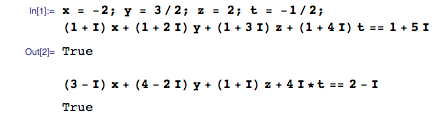
\includegraphics[scale=0.6]{task/2_03/screen1.png}
\subsection{Вывод:}
Мы верно нашли решение системы.

	\section{Задача 2.4}
\subsection{Задание:}

	\section{Задача 2.7}
\subsection{Задание:}
При каких условиях модуль суммы двух комплексных чисел равен разности модулей слагаемых?
\subsection{Решение:}
$
	z_1 = x_1 + i y_1\\
	z_2 = x_2 + i y_2\\
$
Модуль суммы $ z_1 $ и $ z_2 $ это длинна вектора, составленного как векторная сумма $ z_1 $ и $ z_2 $.\\
Таким образом модуль суммы двух комплексных чисел будет равен разности модулей слагаемых когда векторы,
соответствующие $ z_1 $ и $ z_2 $ на плоскости комплексных чисел будут противоположно направленными, то есть
должно выполняться условие:
\\[1em]
$
	\dfrac{x_1}{x_2} = \dfrac{y_1}{y_2} < 0
$
\subsection{Компьютерная проверка в среде Wolfram Mathematica}
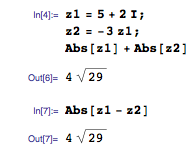
\includegraphics[scale=0.6]{task/2_07/screen1.png}
\subsection{Вывод:}
Мы нашли условие при котором модуль суммы двух комплексных чисел равен разности модулей слагаемых.

	\section{Задача 2.8}
\subsection{Задание:}
Доказать, что если в результате конечного числа рациональных операций (сложение, умножение, вычитание, деление)
выполненых над комплексными числами $ z_1, \dots, z_n $ получается комплексное число $ u $, то в результате выполнения тех же
операций над $ \overline{z_1}, \dots, \overline{z_n} $ получается $ \overline{u} $.
\subsection{Доказательство:}
Пусть $ u_j $ - результат выполнения данных операций с числами $ z_1, \dots, z_j $,
тогда $ u_j = u_{j-1} \; \circ \; z_j $.
\\
Получается что $ u_n = u, \; \overline{u_n} = \overline{u} $.
\\
Докажем что $ \overline{u_j} $ - результат выполнения данных операций с $ \overline{z_1}, \dots, \overline{z_j} $
для каждой из четырёх операций:
\subsection{Сложение:}
$
	\overline{u_j}
	=
	\operatorname{Re} \overline{u_j} + i \operatorname{Im} \overline{u_j}
	=
	\operatorname{Re} u_j - i \operatorname{Im} u_j
	=
	\operatorname{Re} u_{j-1} + \operatorname{Re} z_j - i(\operatorname{Im} u_(j-1) + \operatorname{Im} z_j)
	=
	(\operatorname{Re} u_{j-1} - i\operatorname{Im} u_{j-1}) + (\operatorname{Re} z_j - i\operatorname{Im} z_j)
	=
	\overline{u_{j-1}} + \overline{z_j}
$
\subsection{Вычитание:}
$
	\overline{u_j}
	=
	\operatorname{Re} \overline{u_j} + i \operatorname{Im} \overline{u_j}
	=
	\operatorname{Re} u_j - i \operatorname{Im} u_j
	=
	\operatorname{Re} u_{j-1} - \operatorname{Re} z_j - i(\operatorname{Im} u_(j-1) - \operatorname{Im} z_j)
	=
	(\operatorname{Re} u_{j-1} - i\operatorname{Im} u_{j-1}) - (\operatorname{Re} z_j - i\operatorname{Im} z_j)
	=
	\overline{u_{j-1}} - \overline{z_j}
$
\subsection{Умножение:}
$
	\overline{u_j}
	=
	\operatorname{Re} \overline{u_j} + i \operatorname{Im} \overline{u_j}
	=
	\operatorname{Re} u_j - i \operatorname{Im} u_j
	=
	\operatorname{Re} u_{j-1} \cdot \operatorname{Re} z_j - i(\operatorname{Im} u_{j-1} \cdot \operatorname{Im} z_j)
	=
	\operatorname{Re} u_{j-1} \cdot \operatorname{Re} z_j +
	i(\operatorname{Im} \overline{u_{j-1}} \cdot \operatorname{Im} \overline{z_j})
	=
	\overline{u_{j-1}} \cdot \overline{z_j}
$
\subsection{Деление:}
$
	\overline{u_j}
	=
	\operatorname{Re} \overline{u_j} + i \operatorname{Im} \overline{u_j}
	=
	\operatorname{Re} u_j - i \operatorname{Im} u_j
	=
	\overline{u_{j-1}} / \overline{z_j}
$
\\[2em]
Таким образом в результате тех же операций над $ \overline{z_1}, \dots, \overline{z_n} $ получается $ \overline{u} $.
\subsection{Компьютерная проверка в среде Wolfram Mathematica:}
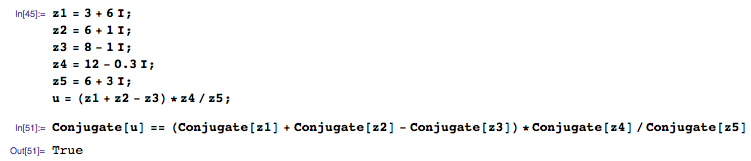
\includegraphics[scale=0.6]{task/2_08/screen1.png}
\\
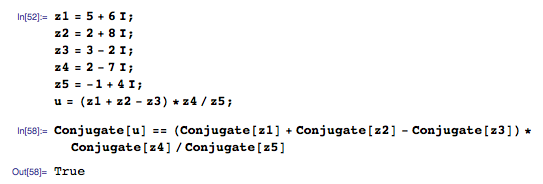
\includegraphics[scale=0.6]{task/2_08/screen2.png}
\subsection{Вывод:}
Утверждение доказано.

	\section{Задача 2.9}
\subsection{Задание:}
Доказать что всякое комплексное $ z \neq -1, |z| = 1 $ представимо в виде $ z = \dfrac{1+it}{1-it}, t \in \mathbb{R} $.
\subsection{Решение:}
$
	\dfrac{1+it}{1-it}
	=
	\dfrac{\sqrt{1+t^2}e^{i\phi}}{\sqrt{1+t^2}e^{-i\phi}}
	=
	e^{2i\phi}
$, где $ \phi = \operatorname{Arg} (1 + it) $
\\
Так как $ |z| = 1 $, $ z $ можно представить как $ e^{i\theta} $, приравняем: $ i\theta = 2i\phi $.
\\
Значит любое комплексное число $ z \neq -1, |z| = 1 $ представимо в виде $ z = \dfrac{1+it}{1-it}, t \in \mathbb{R} $.
\subsection{Выполним проверку в компьютерной среде Wolfram Mathematica:}
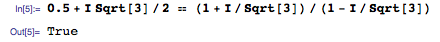
\includegraphics[scale=0.6]{task/2_09/screen.png}
\subsection{Вывод:}
Утверждение доказано и прошло проверку в компьютерной среде.

	\section{Задача 2.10}
\subsection{Задание:}
Визуализировать геометрические места точек комплексной плоскости.
\subsection{Решение:}
a) $ |z| = 1 $
\\
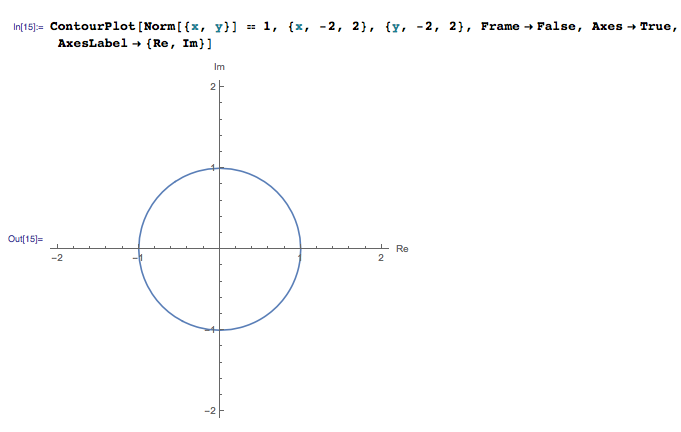
\includegraphics[scale=0.6]{task/2_10/screen1.png}
\\
б) $ \operatorname{Arg} z = \frac{1}{3}\pi $
\\
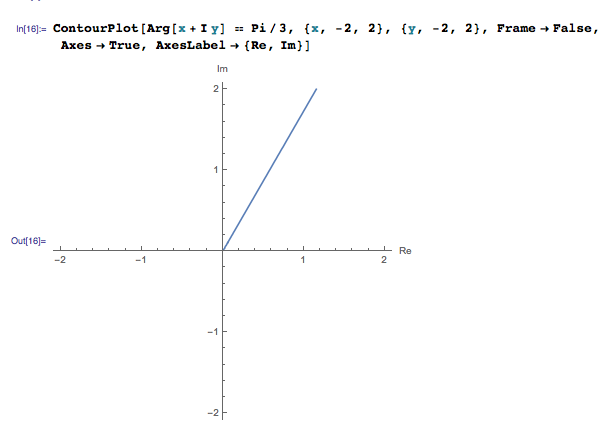
\includegraphics[scale=0.6]{task/2_10/screen2.png}
\\
в) $ |z - 1 - 2i| < 2 $
\\
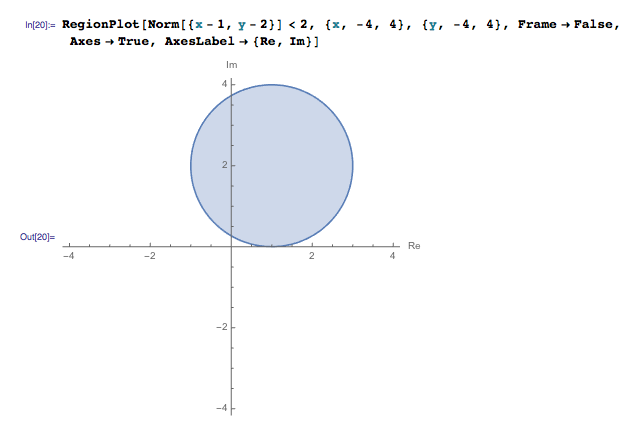
\includegraphics[scale=0.6]{task/2_10/screen3.png}
\\
г) $ |z + 3i| \geq 3 $
\\
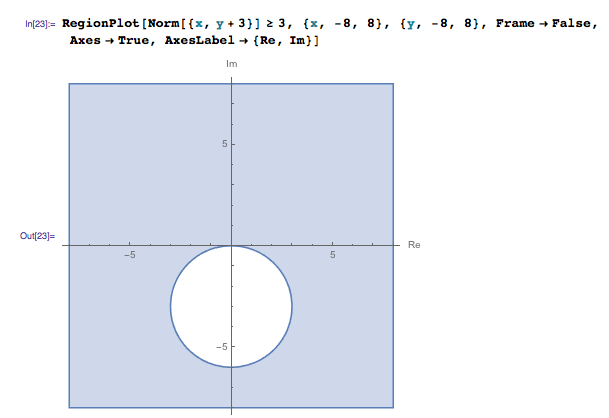
\includegraphics[scale=0.6]{task/2_10/screen4.png}
\\
д)
$
	\begin{cases}
		\operatorname{Re} z > -1
		\operatorname{Im} \leq 2
	\end{cases}
$
\\
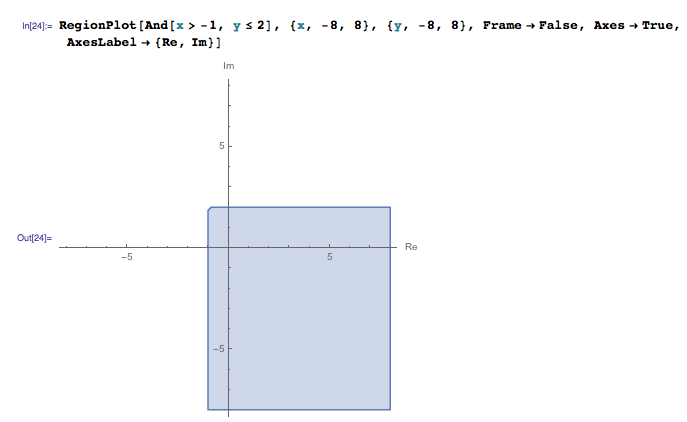
\includegraphics[scale=0.6]{task/2_10/screen5.png}
\\
е)
$ |z+i|=|z-i| $
\\
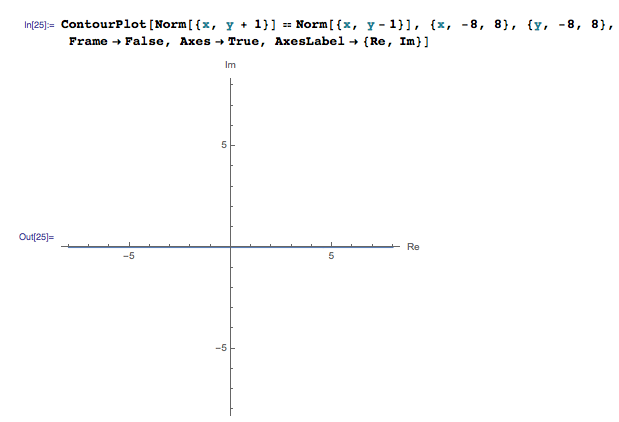
\includegraphics[scale=0.6]{task/2_10/screen6.png}
\\
ж)
$ |\pi - \operatorname{Arg} z| < \dfrac{\pi}{4}, \operatorname{Arg}z \in [0,2\pi) $
\\
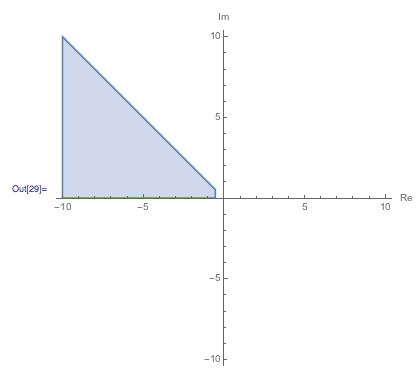
\includegraphics[scale=0.6]{task/2_10/screen7.png}
\\
з)
$
	\begin{cases}
		|z + i| < 1 \\
		-\dfrac{3\pi}{4} \leq \operatorname{Arg} z \leq -\dfrac{pi}{4}
	\end{cases}, \;
	\operatorname{Arg} z \in [-\pi,\pi)
$
\\
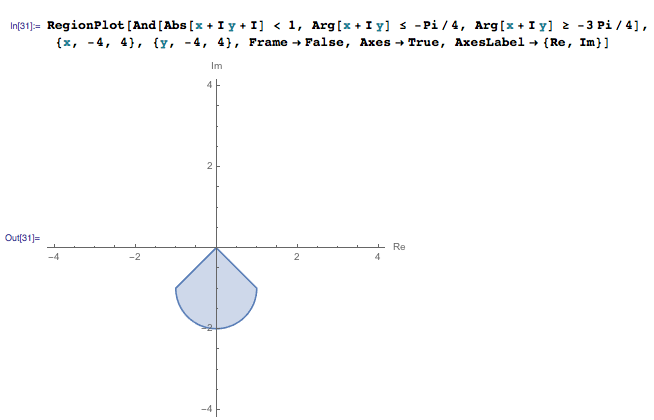
\includegraphics[scale=0.6]{task/2_10/screen8.png}
\\

	\section{Задача 2.11}
\subsection{Задание:}
Вычислить $ \left(1 + \cos \dfrac{pi}{3} + i \sin \dfrac{pi}{3}\right)^7 $.
\subsection{Решение:}
$
	\left(1 + \cos \dfrac{\pi}{3} + i \sin \dfrac{\pi}{3}\right)^7 =
	\left(\dfrac{3}{2} + i \dfrac{\sqrt{3}}{2}\right)^7 =
	\left(\sqrt{3} \cdot \left(\cos \dfrac{\pi}{6} + i \sin \dfrac{\pi}{6}\right)\right)^7 =
	\sqrt{3}^7 \cdot \left(\cos \dfrac{7 \pi}{6} + i \sin \dfrac{7 \pi}{6}\right) =
	3^{\frac{7}{2}} \cdot \left(\dfrac{1}{2} + i \dfrac{\sqrt{3}}{2} \right) =
	\dfrac{27 \sqrt{3}}{2} + i \dfrac{81}{2}
$
\subsection{Проверка в компьютерной среде Wolfram Mathematica:}

	\section{Задача 2.12}
\subsection{Задание:}
Вычислить и визуализировать на комплексной плоскости $ \sqrt[5]{4 - 4i} $.
\subsection{Решение:}
$
	\sqrt[5]{4 - 4i}
	=
	\sqrt[5]{4 \sqrt{2} \left( \cos \dfrac{-\pi}{4} - i \sin \dfrac{-\pi}{4} \right)}
	=
	\sqrt[5]{4 \sqrt{2}} \left( \cos \left( \dfrac{-\pi}{4} + \dfrac{2\pi k}{5} \right) -
	i \sin \left( \dfrac{-\pi}{4} + \dfrac{2\pi k}{5} \right) \right), \; k = \overline{0,4}
$
\subsection{Визуализируем в среде Wolfram Mathematica:}
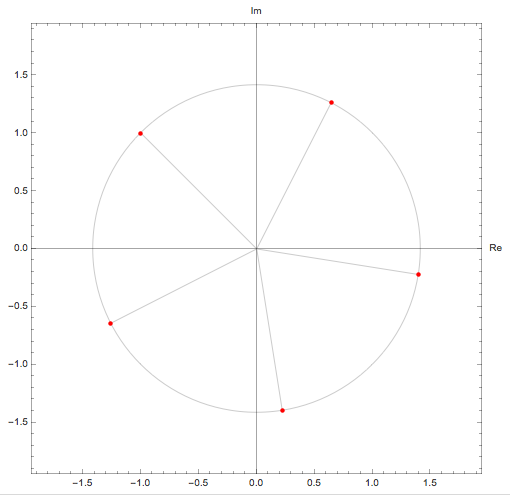
\includegraphics[scale=0.6]{task/2_12/screen.png}

	\section{Задача 2.13}
\subsection{Задание:}
Составить квадратное уравнение с целыми коэффицентами и отрицательным дискриминантом и решить его.
\subsection{Решение:}
Решим уравнение $ x^2 + 2x + 2 = 0 $.
\\
$
	D = 4 - 4 \cdot 1 \cdot 2 = -4
	\\[1em]
	x = \dfrac{-2 \pm \sqrt{-4}}{2}
	\\[1em]
	x = \dfrac{-2 \pm 2i}{2} = -1 \pm i
$
\subsection{Компьютерная проверка в среде Wolfram Mathematica:}
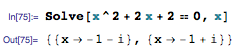
\includegraphics[scale=0.6]{task/2_13/screen.png}

	\section{Задача 2.15}
\subsection{Задание:}
Построить на компьютере графики функций $ u(x,y) = \operatorname{Re} f(z) $, $ v(x,y) = \operatorname{Im} f(z) $
и решить уравнение $ f(z) = -2 $.
\\
$ f(z) = \operatorname{ch} 2z $
\subsection{Решение:}
Построим графики функций $ v $ и $ u $ в среде Wolfram Mathematica:
\\
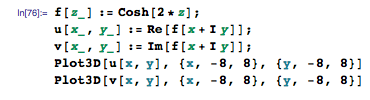
\includegraphics[scale=0.6]{task/2_15/screen1.png}
\\
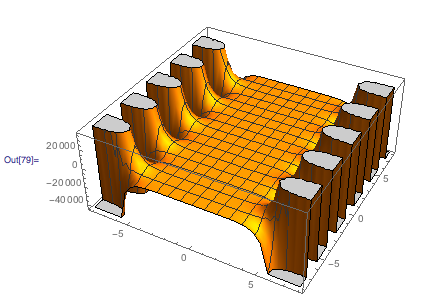
\includegraphics[scale=0.6]{task/2_15/screen2.png}
\\
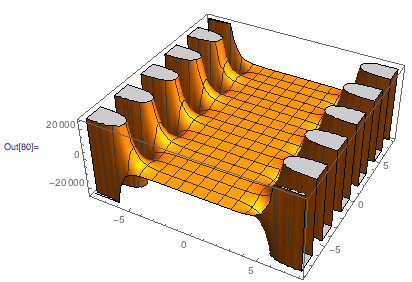
\includegraphics[scale=0.6]{task/2_15/screen3.png}
\\
Решим уравнение $ f(z) = -2 $:\\
$
	\operatorname{ch} 2z = -2
	\\[1em]
	\cos 2y \cdot \ch 2x + i \sin 2y \cdot \sh 2x = -2
	\\[1em]
	\begin{cases}
		\cos 2y \cdot \ch 2x = -2 \\
		\sin 2y \cdot \sh 2x = 0
	\end{cases}
	\\[1em]
$
Рассмотрим два случая: $ \sin 2y = 0 $ и $ \sh 2x = 0 $
\\[1em]
1 случай:
\\[1em]
$
	\sin 2y = 0
	\\[1em]
	\cos 2y = \pm 1
	\\[1em]
	\ch 2x \pm 1 = -2
$

	\section{Задача 2.16}
\subsection{Задание:}
Построить два различных скелетных разложения матрицы $ A $.
\\[1em]
$
	A = \begin{pmatrix}
		-3 & 5 & 4 & -17 & -7 & -11 \\
		1 & 3 & -4 & 1 & -17 & 9 \\
		2 & 0 & -8 & 8 & -16 & 18 \\
		-4 & -6 & 2 & -10 & 22 & -8
	\end{pmatrix}
$
\subsection{Решение:}
Определим линейно независимые строки матрицы $ A $:
\\
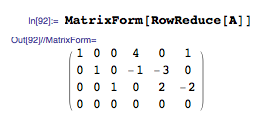
\includegraphics[scale=0.6]{task/2_16/screen1.png}
\\
Первые три строки матрицы $ A $ линейно независимы. Построим матрицу $ C $:
\\[1em]
$
	C =
	\begin{pmatrix}
		-3 & 5 & 4 & -17 & -7 & -11 \\
		1 & 3 & -4 & 1 & -17 & 9 \\
		2 & 0 & -8 & 8 & -16 & 18 \\
	\end{pmatrix}
$
\\[1em]
Из $ A = BC $ найдём матрицу $ B $:
\\[1em]
$
	B = AC^{+} =
	\begin{pmatrix}
		1 & 0 & 0 \\
		0 & 1 & 0 \\
		0 & 0 & 1 \\
		\frac{7}{4} & -\frac{59}{12} & \frac{37}{12}
	\end{pmatrix}
$
Выполним компьютерную проверку разложения в среде Wolfram Mathematica:
\\
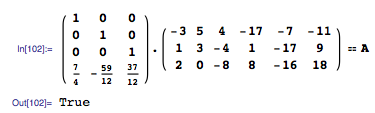
\includegraphics[scale=0.6]{task/2_16/screen2.png}
\\[1em]
Построим второе скелетное разложение $ A $:
\\
Определим линейно независимые столбцы:
\\
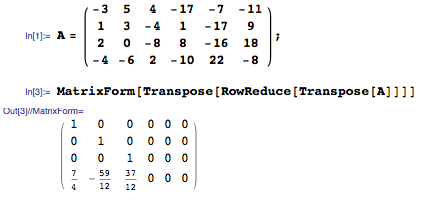
\includegraphics[scale=0.6]{task/2_16/screen3.png}
\\
Видно что первые три столбца матрицы линейно независимы. Составим матрицу $ B $:
\\[1em]
$
	B =
	\begin{pmatrix}
		-3 & 5 & 4 \\
		1 & 3 & -4 \\
		2 & 0 & -8 \\
		-4 & -6 & 2 \\
	\end{pmatrix}
$
\\[1em]
Найдём матрицу $ C $ из $ A = BC $:
\\[1em]
$
	C = B^{+}A =
	\begin{pmatrix}
		1 & 0 & 0 & 4 & 0 & 1 \\
		0 & 1 & 0 & -1 & -3 & 0 \\
		0 & 0 & 1 & 0 & 2 & -2 \\
	\end{pmatrix}
$
\\[1em]
Выполним компьютерную проверку в среде Wolfram Mathematica:
\\
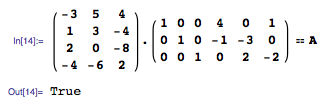
\includegraphics[scale=0.6]{task/2_16/screen4.png}
\subsection{Вывод:}
Мы построили два скелетных разложения матрицы $ A $.

	\section{Задача 2.17}
\subsection{Задание:}
Вычислить ранг матрицы $ A =
	\begin{pmatrix}
			11 & 0 & 11 & 8 & 0 & 4 & 8 \\
			15 & 0 & 0 & -3 & -15 & 0 & -6 \\
			13 & -9 & 0 & 14 & 0 & 10 & 0 \\
			-1 & 0 & -7 & 0 & 12 & -15 & 14 \\
			-7 & 0 & -2 & 0 & 0 & 12 & 0 \\
	\end{pmatrix}
$
\subsection{Решение:}
Приведём матрицу $ A $ к ступенчатому виду с помощю элементарных преобразований:
\\
$
\begin{pmatrix}
	11 & 0 & 11 & 8 & 0 & 4 & 8 \\
	15 & 0 & 0 & -3 & -15 & 0 & -6 \\
	13 & -9 & 0 & 14 & 0 & 10 & 0 \\
	-1 & 0 & -7 & 0 & 12 & -15 & 14 \\
	-7 & 0 & -2 & 0 & 0 & 12 & 0 \\
\end{pmatrix}
\sim
\begin{pmatrix}
	15 & 0 & 0 & -3 & -15 & 0 & -6 \\
	11 & 0 & 11 & 8 & 0 & 4 & 8 \\
	13 & -9 & 0 & 14 & 0 & 10 & 0 \\
	-1 & 0 & -7 & 0 & 12 & -15 & 14 \\
	-7 & 0 & -2 & 0 & 0 & 12 & 0 \\
\end{pmatrix}
\sim
\\
\begin{pmatrix}
	15 & 0 & 0 & -3 & -15 & 0 & -6 \\
	0 & 0 & 11 & \frac{51}{5} & 11 & 4 & \frac{62}{5} \\
	13 & -9 & 0 & 14 & 0 & 10 & 0 \\
	-1 & 0 & -7 & 0 & 12 & -15 & 14 \\
	-7 & 0 & -2 & 0 & 0 & 12 & 0 \\
\end{pmatrix}
\sim
\begin{pmatrix}
	5 & 0 & 0 & -1 & -5 & 0 & -2 \\
	0 & 0 & 11 & \frac{51}{5} & 11 & 4 & \frac{62}{5} \\
	13 & -9 & 0 & 14 & 0 & 10 & 0 \\
	-1 & 0 & -7 & 0 & 12 & -15 & 14 \\
	-7 & 0 & -2 & 0 & 0 & 12 & 0 \\
\end{pmatrix}
\sim
\\
\begin{pmatrix}
	5 & 0 & 0 & -1 & -5 & 0 & -2 \\
	0 & 0 & 55 & 51 & 55 & 20 & 62 \\
	13 & -9 & 0 & 14 & 0 & 10 & 0 \\
	-1 & 0 & -7 & 0 & 12 & -15 & 14 \\
	-7 & 0 & -2 & 0 & 0 & 12 & 0 \\
\end{pmatrix}
\sim
\begin{pmatrix}
	5 & 0 & 0 & -1 & -5 & 0 & -2 \\
	0 & 0 & 55 & 51 & 55 & 20 & 62 \\
	0 & -9 & 0 & \frac{83}{5} & 13 & 10 & \frac{26}{5} \\
	-1 & 0 & -7 & 0 & 12 & -15 & 14 \\
	-7 & 0 & -2 & 0 & 0 & 12 & 0 \\
\end{pmatrix}
\sim
\\
\begin{pmatrix}
	5 & 0 & 0 & -1 & -5 & 0 & -2 \\
	0 & 0 & 55 & 51 & 55 & 20 & 62 \\
	0 & -45 & 0 & 83 & 65 & 50 & 26 \\
	-1 & 0 & -7 & 0 & 12 & -15 & 14 \\
	-7 & 0 & -2 & 0 & 0 & 12 & 0 \\
\end{pmatrix}
\sim
\begin{pmatrix}
	5 & 0 & 0 & -1 & -5 & 0 & -2 \\
	0 & 0 & 55 & 51 & 55 & 20 & 62 \\
	0 & -45 & 0 & 83 & 65 & 50 & 26 \\
	0 & 0 & -7 & -\frac{1}{5} & 11 & -15 & \frac{68}{5} \\
	-7 & 0 & -2 & 0 & 0 & 12 & 0 \\
\end{pmatrix}
\sim
\\
\begin{pmatrix}
	5 & 0 & 0 & -1 & -5 & 0 & -2 \\
	0 & 0 & 55 & 51 & 55 & 20 & 62 \\
	0 & -45 & 0 & 83 & 65 & 50 & 26 \\
	0 & 0 & 35 & 1 & -55 & 75 & -68 \\
	-7 & 0 & -2 & 0 & 0 & 12 & 0 \\
\end{pmatrix}
\sim
\begin{pmatrix}
	5 & 0 & 0 & -1 & -5 & 0 & -2 \\
	0 & 0 & 55 & 51 & 55 & 20 & 62 \\
	0 & -45 & 0 & 83 & 65 & 50 & 26 \\
	0 & 0 & 35 & 1 & -55 & 75 & -68 \\
	0 & 0 & -2 & -\frac{7}{5} & -7 & 12 & -\frac{14}{5} \\
\end{pmatrix}
\sim
\\
\begin{pmatrix}
	5 & 0 & 0 & -1 & -5 & 0 & -2 \\
	0 & 0 & 55 & 51 & 55 & 20 & 62 \\
	0 & -45 & 0 & 83 & 65 & 50 & 26 \\
	0 & 0 & 35 & 1 & -55 & 75 & -68 \\
	0 & 0 & 10 & 7 & 35 & -60 & 14 \\
\end{pmatrix}
\sim
\begin{pmatrix}
	5 & 0 & 0 & -1 & -5 & 0 & -2 \\
	0 & -45 & 0 & 83 & 65 & 50 & 26 \\
	0 & 0 & 55 & 51 & 55 & 20 & 62 \\
	0 & 0 & 35 & 1 & -55 & 75 & -68 \\
	0 & 0 & 10 & 7 & 35 & -60 & 14 \\
\end{pmatrix}
\sim
\\
\begin{pmatrix}
	5 & 0 & 0 & -1 & -5 & 0 & -2 \\
	0 & 45 & 0 & -83 & -65 & -50 & -26 \\
	0 & 0 & 55 & 51 & 55 & 20 & 62 \\
	0 & 0 & 0 & 346 & 990 & -685 & 1182 \\
	0 & 0 & 10 & 7 & 35 & -60 & 14 \\
\end{pmatrix}
\sim
\begin{pmatrix}
	5 & 0 & 0 & -1 & -5 & 0 & -2 \\
	0 & 45 & 0 & -83 & -65 & -50 & -26 \\
	0 & 0 & 55 & 51 & 55 & 20 & 62 \\
	0 & 0 & 0 & 346 & 990 & -685 & 1182 \\
	0 & 0 & 0 & -5 & 55 & -140 & 6 \\
\end{pmatrix}
\sim
\\
\begin{pmatrix}
	5 & 0 & 0 & -1 & -5 & 0 & -2 \\
	0 & 45 & 0 & -83 & -65 & -50 & -26 \\
	0 & 0 & 55 & 51 & 55 & 20 & 62 \\
	0 & 0 & 0 & 346 & 990 & -685 & 1182 \\
	0 & 0 & 0 & 0 & 2180 & -4715 & 726 \\
\end{pmatrix}
$
\\
Из приведённой к ступенчатому виду матрицы видно что $ rank A = 51 $.
\subsection{Выполним компьютерную проверку в среде Wolfram Mathematica:}
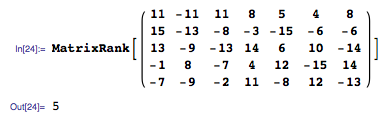
\includegraphics[scale=0.6]{task/2_17/screen.png}

	\section{Задача 2.18}
\subsection{Задание:}
Построить графический образ зависимости $ \operatorname{Rg} A = f(x) $, где
\\[1em]
$
	A(x) =
	\begin{pmatrix}
		3 & 1 & 1 & 4 \\
		x & 4 & 10 & 1 \\
		1 & 7 & 17 & 3 \\
		2 & 2 & 4 & 1
	\end{pmatrix}
$
\subsection{Решение:}
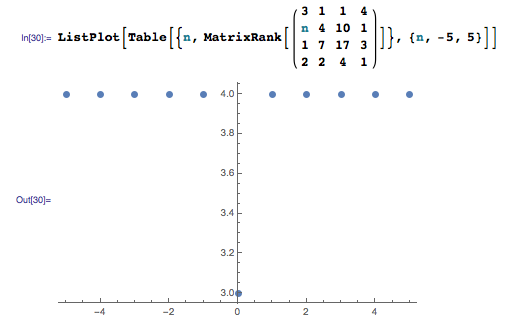
\includegraphics[scale=0.6]{task/2_18/screen.png}
\\
Видно что ранг достигает значения $ 4 $, так как в $ A $ только $ 4 $ столбца и строки, $ \max \operatorname{Rg} A = 4 $.

	\section{Задача 2.21}
\subsection{Задание:}
Как может изменится ранг матрицы в результате вычёркивания из неё одной строки (столбца)?
\subsection{Решение:}
При вычёркивании из матрицы строки или столбца ранг не изменится
если вычеркнутая строка линейно зависима, иначе ранг уменьшится на 1.

	\section{Задача 2.22}
\subsection{Задание:}
Доказать, что любую матрицу ранга $ r $ можно представить в виде суммы $ r $
матриц ранга 1, но нельзя представить в виде суммы менее чем $ r $ таких матриц.
\subsection{Доказательство:}
Пусть дана матрица $ A \in M(n, m) $, где первые $ r $ строк являются линейно независимыми, а все последующие являются их
линейными комбинациями. Тогда $ A $ можно представить как сумму
$ A_1, A_2, \dots, A_r $, где
\\[1em]
$
	A_i =
	\begin{pmatrix}
		0 & 0 & \cdots & 0 & 0 \\
		\vdots & \vdots & \ddots & \vdots & \vdots \\
		a_{i1} & a_{i2} & \cdots & a_{i(m-1)} & a_{i(m)} \\
		\vdots & \vdots & \ddots & \vdots & \vdots \\
		k_{j1} & k_{j2} & \cdots & k_{j(m-1)} & k_{j(m)} \\
		\vdots & \vdots & \ddots & \vdots & \vdots \\
		k_{n1} & k_{n2} & \cdots & k_{n(m-1)} & k_{n(m)} \\
	\end{pmatrix}
	, k_{jl}
$ - коэффиценты линейных комбинаций линейно зависимых строк.
\\[1em]
Так как ранг суммы матриц может быть больше суммы рангов этих матриц, количество слагаемых
с рангом $ 1 $ не может быть меньше ранга суммы $ A $.

	\section{Задача 2.23}
\subsection{Задание:}
а) Выяснить, образует ли множество функций, ограниченных на некотором $ [a, b] $
линейное пространство относительно обычных операций сложения и умножения на число.
\\
б) Выяснить, является ли линейным подпространством множество векторов плоскости, по модулю не превосходящих 1.
\\
в) Выяснить, является ли множество верхних треугольных матриц порядка $ n $ линейным подпространством
в пространстве всех квадратных матриц поряжка $ n $, и если является, то найти его размерность.
\\
г) Выяснить, является ли линейным подпространством множество векторов в $ n $ - мерном пространстве,
сумма координат которых равна 0, и если является, то найти его размерность.
\subsection{Решение:}
а) Выяснить, образует ли множество функций, ограниченных на некотором $ [a, b] $
линейное пространство относительно обычных операций сложения и умножения на число.
\\[1em]
Пусть дано множество функций $ \mathbb{F} $, ограниченных на $ [a, b] $ и $ f(x), g(x) \in \mathbb{F} $.
Зададим операции сложения $ (f + g)(x) = f(x) + g(x) $,
умножения на число $ (\lambda f)(x) = \lambda (f(x)), \lambda \in \mathbb{R} $.
\\
Докажем что $ f(x) + g(x) \in \mathbb{F} $: функции $ f(x) $ и $ g(x) $ ограниченны сверху на $ [a, b] $,
значит существуют точные верхние грани этих функций $ F, G $ соответственно, тогда точная верхняя грань функции $ f(x) + g(x) $
 - $ F + G $, поскольку она существует, функция $ f(x) + g(x) $ ограничена сверху.
Аналогично доказывается что функция $ f(x) + g(x) $ ограничена снизу. Значит $ f(x) + g(x) \in \mathbb{F} $.
\\
Докажем что $ \lambda f(x) \in \mathbb{F} $: $ f(x) $ ограничена сверху, $ \Rightarrow \exists F $ - верхняя грань $ f(x) $.
$ f(x) < F \Rightarrow \lambda f(x) < \lambda F $. Значит $ \lambda f(x) $ ограничена сверху. Аналогично доказывается что
$ \lambda f(x) $ ограничена снизу. Значит $ \lambda f(x) \in \mathbb{F} $.
\\
Проверим аксиомы линейного пространства:
\\[1em]
$
	(f + g)(x) = f(x) + g(x) = g(x) + f(x) = (g + f)(X)\\[1em]
	(f + g)(x) + m(x) = f(x) + g(x) + m(x) = f(x) + (g + m)(x) \\[1em]
	\exists \theta : \theta (x) = 0, (f + \theta)(x) = f(x) + \theta(x) = f(x)\\[1em]
	\exists -f(x) : -f(x) + f(x) = \theta\\
	(-f + f)(x) = -f(x) + f(x) = (-1)f(x) + f(x) = \theta\\[1em]
	\lambda(f + g)(x) = \lambda f(x)  + \lambda g(x)  = (\lambda f + \lambda g)(x)\\[1em]
	(\alpha + \beta)f(x) = \alpha f(x) + \beta f(x) = (\alpha f + \beta f)(x)\\[1em]
	\alpha(\beta f(x)) = (\alpha \beta)f(x) = (\alpha \beta f)(x)\\[1em]
	(1 \cdot f)(x) = 1 \cdot f(x) = f(x)\\[1em]
$
Значит множество $ \mathbb{F} $ - линейное пространство.
\\[2em]
б) Выяснить, является ли линейным подпространством множество векторов плоскости, по модулю не превосходящих 1.
\\[1em]
Пусть $ L $ - множество векторов плоскости, по модулю не превосходящих 1, $ a = (0, 1), \; b = (1, 0) $.
\\
$ a, b \in L $, когда $ a + b \notin L $, значит $ L $ не является линейным пространством.
\\[2em]
в) Выяснить, является ли множество верхних треугольных матриц порядка $ n $ линейным подпространством
в пространстве всех квадратных матриц поряжка $ n $, и если является, то найти его размерность.
\\[1em]
При сложении двух верхних треугольных матриц получается верхняя треугольная матрица.
При умножении верхней треугольной матрицы на число получается верхняя треугольная матрица.
Так как аксиомы выполняются для множества квадратных матриц порядка $ n $, они будут выполнятся
и для верхних треугольных матриц. Размерность подпространства верхних треугольных матриц будет равна
$ \sum \limits_{i=1}^n i $.
\\[2em]
г) Выяснить, является ли линейным подпространством множество векторов в $ n $ - мерном пространстве,
сумма координат которых равна 0, и если является, то найти его размерность.
\\[1em]
При сложении двух таких векторов получается вектор сумма координат которого равна нулю.
При умножении такого вектора на число получается вектор сумма координт котороо тоже равна нулю.
Аксиомы выполняются для всех векторов. Так как одна координата равна сумме других взятой с противоположным знаком, размерность
такого пространства будет равна $ n - 1 $.


\end{document}
